\documentclass[a4paper,fleqn,12pt]{article}

%%%%%%%%%%%%%%%%%%%%


\usepackage[]{geometry}
\usepackage[latin1, utf8]{inputenc}
\usepackage[UKenglish]{babel}
\usepackage[UKenglish]{isodate}
\usepackage{amsmath}
\usepackage{amsfonts}
\usepackage{amssymb}
\usepackage{amsthm}
\usepackage{graphicx}
\usepackage{chngpage}
\usepackage{calc}
\PassOptionsToPackage{hyphens}{url}
\usepackage{hyperref}
\usepackage[nameinlink]{cleveref}
\usepackage{fancyhdr}
\usepackage{titletoc}
\usepackage[explicit]{titlesec}
\usepackage[square, numbers]{natbib}
\usepackage[dvipsnames]{xcolor}
\usepackage[sc]{mathpazo}
\linespread{1.05}
\usepackage[T1]{fontenc}
\usepackage[backgroundcolor=gray!5, hidealllines=true, roundcorner=10pt]{mdframed}
\usepackage{multirow}
\usepackage{subfig}
\usepackage{pgf-pie}
\hypersetup{
	colorlinks=true,
	linkcolor=black,
	urlcolor=black,
	citecolor=black
}
\usepackage[nomap]{FiraMono}
\usepackage{pdfpages}

\setlength{\parindent}{0mm}
\setlength{\parskip}{\medskipamount}
\renewcommand\baselinestretch{1.2}

\cleanlookdateon{}

\makeatletter
\newcommand{\@assignment}[0]{Assignment}
\newcommand{\assignment}[1]{\renewcommand{\@assignment}{#1}}
\newcommand{\@supervisor}[0]{}
\newcommand{\supervisor}[1]{\renewcommand{\@supervisor}{#1}}
\newcommand{\@yearofstudy}[0]{}
\newcommand{\yearofstudy}[1]{\renewcommand{\@yearofstudy}{#1}}
\newcommand{\txt}[1]{\mintinline{text}{#1}}
\newcommand{\scala}[1]{\mintinline{scala}{#1}}
\makeatletter

\newtoggle{IsDissertation}


%%%%%%%%%%%%%%%%%%%%%%%%%%%%%%%%%%%%%%%%%%%%%%%%%%%%%%%%%%%%%%%%%%%%%%%%%%%%%%%
%% Project-specific configuration
%%%%%%%%%%%%%%%%%%%%%%%%%%%%%%%%%%%%%%%%%%%%%%%%%%%%%%%%%%%%%%%%%%%%%%%%%%%%%%%

\author{Your name}
\title{Project title}
% \supervisor{Your supervisor's name}
% \yearofstudy{3\textsuperscript{rd}}

%%%%%%%%%%%%%%%%%%%%%%%%%%%%%%%%%%%%%%%%%%%%%%%%%%%%%%%%%%%%%%%%%%%%%%%%%%%%%%%


\assignment{Project specification}

%%%%%%%%%%%%%%%%%%%%

\pagestyle{plain}
\renewcommand{\headrulewidth}{0.0pt}

\makeatletter
\fancypagestyle{plain}{
	\fancyhf{}
    \fancyfoot[C]{\thepage}
}
\makeatother

%%%%%%%%%%%%%%%%%%%%
\begin{document}

\makeatletter
\begin{titlepage}

    % do not show the assignment name for the dissertation
    \iftoggle{IsDissertation}
    {
        \textbf{\Huge \@title} \\[1.5cm]
    }
    {
        \textbf{\Huge \@title} \\
        \Large \@assignment \\[1.5cm]
    }
    \Large \textbf{\@author} \\
    Department of Computer Science \\
    University of Warwick \\

    % include the supervisor and year of study if the are specified and its the disseration
    \iftoggle{IsDissertation}{
        \ifdefempty{\@supervisor}{}{
            Supervised by \@supervisor \\
        }\ifdefempty{\@yearofstudy}{}{
            Year of Study: \@yearofstudy \\
        }
    }{}

    \vfill

    % include the current date for the dissertation
    \iftoggle{IsDissertation}{\today}{}

    \begin{adjustwidth}{-\oddsidemargin-1in}{-\rightmargin}
        \centering
        
\includegraphics[width=\paperwidth]{../common/line.png}
    \end{adjustwidth}

    \vspace*{-3.5cm}

\end{titlepage}
\makeatother


\pagestyle{plain}

\section{Introduction}
Traditionally, general-purpose microcontrollers necessitate the inclusion of a wide variety of hardware interfaces such as UART, SPI, and I2C to interface with a broad range of peripherals. Each of these interfaces has different hardware requirements, and is costly in development time, chip area, and system power. These interfaces are often emulated over general-purpose I/O interfaces using software techniques, but such techniques are usually inefficient and have poor performance.

The aim of this project is to develop state machine-based programmable I/O blocks which are able to emulate any hardware interface or implement any communication protocol, via programming using a small assembly-like DSL. These blocks will then be integrated with open-source RISC-V cores to create a flexible and compact microcontroller, ideal for use in low power, low cost embedded applications. This microcontroller would be applicable for any use in which traditional hardware interfaces are needed, but also for applications which have specific or highly custom I/O requirements, without the need for programmable logic (as is found in FPGAs) or custom hardware.

\section{Background}

The primary purpose of embedded systems and microcontrollers is usually to interact with the real world via sensors, actuators, LEDs, speakers, etc, but communicating with such hardware can be difficult due to the need for high frequencies and precise timing requirements. Computers and microcontrollers include dedicated hardware for high-speed interfaces: SATA and PCIe are common in desktop-class hardware and used to interface with consumer hardware, but interfaces such as UART, SPI, I2C, PWM and I2S are more general-purpose buses usually found in microcontrollers and designed for use with a wide variety of electronics devices. These protocols are also simpler and cheaper (in terms of power, space and money) to implement than the likes of SATA, making them ideal for lower-cost microcontrollers. All of these interfaces have different hardware and software requirements, and the cost and complexity associated with implementing all of these in a device may mean you end up with lots of interfaces you don't need, or not enough of a single type of interface.

A common alternative to using dedicated hardware is to use the CPU to control GPIO (General Purpose I/O) pins, implementing the control and timing processes in software: a process known as 'bit-banging'. However, general-purpose software processors are generally not designed to do this, and maintaining precise timing requirements at high speed is very hard, especially when the processor has other work to do. For example, SPI can run at up 100MHz, a speed which is impossible to maintain on most consumer microcontrollers, especially lower-power ones \citep{picosdk}.

The usual solution to custom interface requirements is FPGAs (Field Programmable Gate Arrays): programmable hardware devices that can be configured by an engineer to implement whatever hardware they wish. These are very flexible but come at a high price, and there is also still the need for software processor alongside it. 'Soft' CPU cores can be implemented in FPGAs alongside other hardware devices, and some embedded systems such as the Xilinx Zynq SoCs combine traditional ARM processing cores with programmable logic slices, connected over various buses \citep{zynq}. FPGAs also present a very different programming model, as programmers are not writing software but designing hardware.


\begin{figure}[b!]
    \centering
    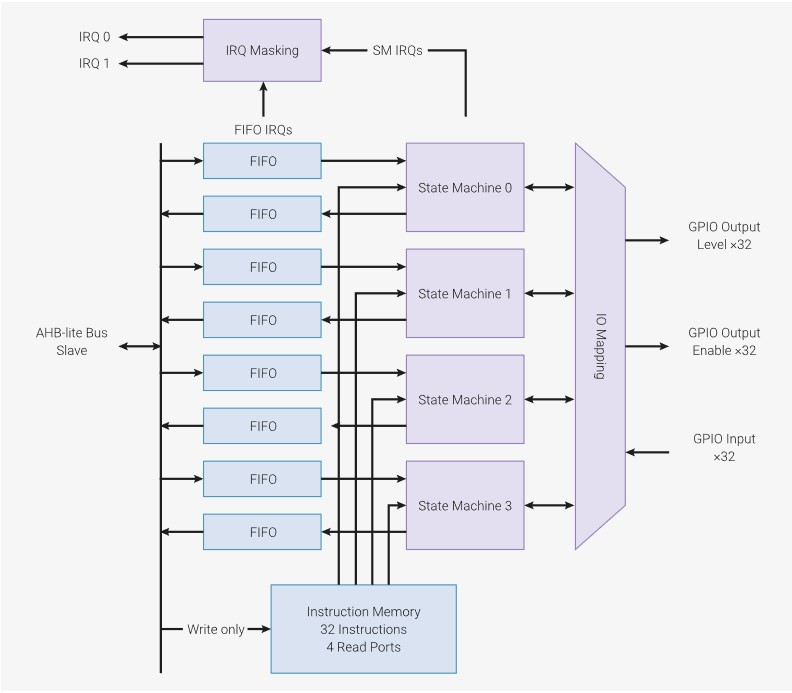
\includegraphics[width=0.7\textwidth]{../img/pio-block.jpg}
    \caption{A PIO block from the RP2040 \citep{rp2040}}
    \label{fig:pio-block}
\end{figure}


It is this problem that I intend to tackle: developing a flexible, low cost, easy to use hardware interface for embedded systems. The inspiration for this comes from the RP2040: a dual-core ARM-based microcontroller designed by Raspberry Pi Ltd released in 2021. The flagship feature of the RP2040 is PIO (Programmable I/O blocks), which are as I have described in my introduction. Two PIO blocks are included in the RP2040, each of which includes 4 state machines, as shown in figure \ref{fig:pio-block}.

The PIO state machines are designed specifically for I/O, able to move data with the speed and timing precision required for high-speed serial I/O interfaces such as SPI, UART and even VGA/DPI. As shown in figure \ref{fig:pio-sm}, each state machine consists of:

\begin{itemize}
    \item Two 32-bit shift registers
    \item Two 32-but scratch registers
    \item A fractional clock divider
    \item Flexible GPIO pin mapping
    \item 4x32 bit Rx/Tx FIFOs connected to the system bus, able to sustain up to one word per clock to/from DMA
\end{itemize}

\begin{figure}[H]
    \centering
    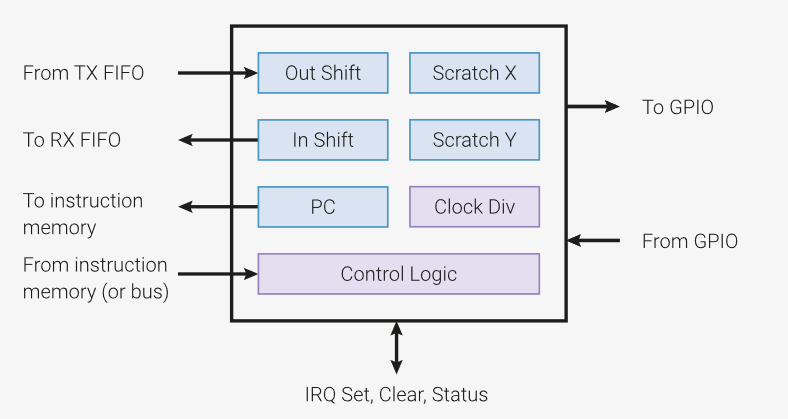
\includegraphics[width=0.7\textwidth]{../img/rp2040-state-machine.png}
    \caption{An overview of a PIO State Machine \citep{rp2040}}
    \label{fig:pio-sm}
\end{figure}

The state machines are programmed using \texttt{pioasm} (PIO Assembly). An example program is shown in listing \ref{pioasm} to output a simple square wave.

\begin{listing}[b]
    \vspace{0.5cm}
    \begin{minted}{asm}
    .program squarewave
    set pindirs, 1   ; Set pin to output
again:
    set pins, 1 [1]  ; Drive pin high then delay for one cycle
    set pins, 0      ; Drive pin low
    jmp again        ; Set PC to label `again`
    \end{minted}
    \caption{PIO Assembly to output a square wave \citep{rp2040}}
    \label{pioasm}
\end{listing}

Another similar hardware device from which I may draw inspiration is the Time Processor Unit (TPU), a device found in some Motorola microcontrollers. The TPU is a coprocessor engine designed to handle complex timing and I/O tasks, independently of the CPU. The TPU consists of a microengine and scheduler for precision timing and execution of instructions, and up to 16 timer channels connected to external pins. Communication with the rest of the system is done via a shared dual-port RAM. Similar to the RP2040, it works by processing and executing microinstructions written by the programmer. Figure \ref{fig:tpu} shows a high-level block diagram of the TPU \citep{tpu}.

\begin{figure}[]
    \centering
    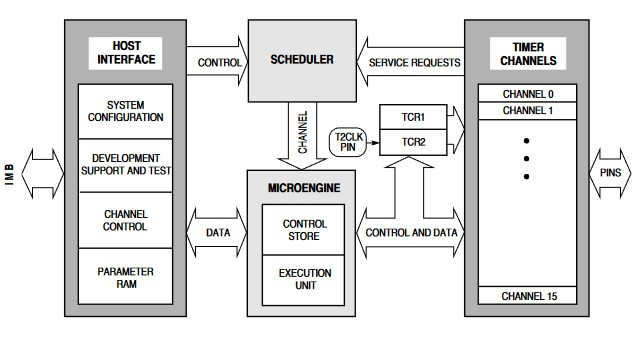
\includegraphics[width=0.8\textwidth]{../img/tpu.jpg}
    \caption{An overview of a Time Processor Unit \citep{tpu}}
    \label{fig:tpu}
\end{figure}

Another major component of this project will be Chisel and Rocket Chip. Chisel is a hardware description language embedded in the Scala programming language. Traditional HDLs such as Verilog and VHDL were originally designed for simulation, and were only later adopted for use in hardware synthesis. Such languages are also very old, and can be unergonomic when contrasted with modern programming languages and tooling. Chisel takes advantage of the modern features and functional style of Scala, and all the tooling and ecosystem around the JVM to provide a much more ergonomic and extensible development process and experience\citep{chisel}. I intend to explore Chisel as an alternative to Verilog for hardware design, evaluating what aspects of the development process it can improve, and also how easy it is to integrate into traditional FPGA workflows.

Rocket Chip is an open source SoC generator that leverages Chisel to provide a library of hardware generators for RISC-V cores, caches and SoC interconnect. It's extensive parametrisation makes it flexible, and can be used to build anything from embedded microcontrollers to multi-core server class CPUs \citep{rocketchip}. It is easy to add custom components to Rocket Chip, which makes it an ideal candidate for experimentation, and build out to custom I/O devices into a fully-fledged SoC.

\section{Objectives}
My goal is to expand on the prior work of current hardware devices and use Chisel to build open source programmable I/O devices, integrated with Rocket RISC-V cores to create a complete microcontroller. Implementation will target FPGAs, as this allows for rapid prototyping and easy implementation and testing of hardware. The requirements for my I/O device are summarised below.

\begin{itemize}
    \item The device should be implemented using Chisel
    \item The device should have a small instruction memory for holding programs
    \item The device should be programmable using a simple DSL
    \item The device should execute instructions from it's memory in a standard fetch-decode-execute fashion
    \item Instructions should execute within a single cycle
    \item Instructions should either push data to the output pins, or shift data in from the pins 
    \item The device should contain an interface for streaming data to/from a host device or external memory
    \item The device should be able to flexibly map inputs and outputs to external GPIO pins on the FPGA
\end{itemize}

The secondary goal, once the HDL implementation is complete and all requirements above are fulfilled, is to build a microcontroller integrating the devices using Rocket Chip. The requirements for this are summarised below.

\begin{itemize}
    \item The microcontroller should contain at least one CPU core, programmable using the RISC-V ISA
    \item The microcontroller should be capable of executing instructions independently from the device
    \item The microcontroller should connect to the device over some bus, and be able to share data via a common memory or some other bus communication protocol
    \item The microcontroller should be capable of acting as a host for the devices, controlling initialisation and handling interrupts 
    \item The microcontroller should be compact and efficient, using as little FPGA resources and power as possible.
\end{itemize}

\section{Timeline}

Table \ref{tab:timeline} gives a rough timeline for my project. Each of the tasks in the table is dependent upon the previous. There are a few notes of context for this:

\begin{itemize}
    \item Week 1 is the start of Term 1
    \item Week 15 is the start of Term 2
    \item The final report is due in Week 31
    \item I have planned to do more work in Term 2, as I am taking more modules in term 1 than term 2.
\end{itemize}


\begin{table}[h!]
    \centering
    \begin{tabular}{|c|l|}
        \hline
        \textbf{Week(s)} & \textbf{Task}                                                       \\ \hline
        1-2              & Background research                                                 \\ \hline
        3-5              & Implement proof of concept I/O device in CHISEL                     \\ \hline
        6-8              & Lay out high-level block design                                     \\ \hline
        8-11             & Extend proof of concept into project skeleton based on block design \\ \hline
        12-18            & Write HDL code, implementing and testing one module at a time       \\ \hline
        19               & Develop and run integration tests in simulation                     \\ \hline
        20-21            & Use Rocket Chip to integrate device with RISC-V cores               \\ \hline
        22-24            & Load microcontroller onto FPGA and run tests                        \\ \hline
        25-31            & Write report                                                        \\ \hline
    \end{tabular}
    \caption{Project Timeline}
    \label{tab:timeline}
\end{table}

\section{Methodology}
This project is very practical, and the bulk of my time will be spent writing and testing HDL code. As such, an appropriate software engineering methodology is required. My approach will be very plan based, first laying out a high-level block design on paper, then moving to lay out skeleton HDL code, then writing the code one module at a time. Any iteration on the design will require going back to the block design, necessitating a waterfall-style approach to development. When it comes to implementing each individual module I intend to take the opposite approach with a very flexible, agile methodology based on extreme programming with constant iteration and testing. This is made easy by the fact that I am working alone, and also do not have any customers or stakeholders besides myself.

When it comes to testing, I intend to utilised test-driven development (TDD) heavily. Functional verification of hardware is very important, as it's much harder to tell to debug hardware designs than software, and synthesising and testing hardware on an FPGA can be time consuming. ChiselTest is a batteries-included a formal verification framework for Chisel that integrates with ScalaTest, the standard Scala testing framework, and with FIRRTL, Chisel's backend RTL compiler.  The idea of TDD is that I can use ChiselTest to write the testbench before or alongside the module, and then implement the module with confidence that it works as intended. A comprehensive test suite will allow me to develop iteratively and with confidence. \citep{chiselverification}


\section{Resources}
There are a few hardware and software resources I'll need access to for completing the project. These are outlined in table \ref{tab:resources}, along with explanations for each. Free, open source software tools and libraries such as Chisel, Scala, and Rocket Chip are not included as they are freely and readily available due to their open source licenses.

\begin{table}[h!]
    \centering
    \begin{tabular}{|p{0.2\textwidth}|p{0.35\textwidth}|p{0.35\textwidth}|}
        \hline
        \textbf{Resource}          & \textbf{Explanation}                                                            & \textbf{Notes}                                                                                                                                   \\ \hline
        FPGA development board     & Used as a synthesis target for the HDL, and for testing the I/O devices and SoC & I have a \href{https://digilent.com/reference/programmable-logic/nexys-a7/start}{Digilent Nexys A7 Board} on loan from the School of Engineering \\ \hline
        Peripheral devices         & Used for testing a variety of interfaces and protocols with the  I/O devices    & I intend to purchase some sensors and LEDs that are designed to connect to the FPGA board                                                        \\ \hline
        Xilinx Vivado Design Suite & FPGA development toolchain and IDE needed for working with FPGA                 & The School of Engineering has an education license                                                                                               \\ \hline
        Workstation PC             & Needed for running Vivado and connection to FPGA board                          & I have a sufficiently capable Linux workstation, and I also have access to DCS \& SoE computer labs.                                             \\ \hline
    \end{tabular}
    \caption{Project Resources}
    \label{tab:resources}
\end{table}


\section{Legal, Social, Ethical and Professional Issues}

There are some legal issues to consider, as I am developing hardware similar to other commercial hardware. Care must be taken to ensure that the devices I develop are sufficiently distinct from existing implementations, as not to infringe upon the terms of any licensing or patent issues. However, I do not believe this will be a problem for two reasons: my implementation will likely be very rudimentary in comparison, and I do not intend to sell, manufacture, or otherwise profit off any of the outcomes of this project.

Other social, ethical and professional issues have been considered, and there is nothing else to note. As this project does not require working with people, no ethical consent is required.

\bibliographystyle{../common/plainnat}
\bibliography{../common/bibliography}

\end{document}
